\documentclass{article}
\usepackage[utf8]{inputenc}
\usepackage{graphicx}
\graphicspath{ {../figs/} }

\title{Problem Set 2: International Trade and Payment Theory (ECON 8402)}
\author{Teerat Wongrattanapiboon}
\date{27 November 2021}

\begin{document}

	\maketitle
	
	\noindent\textbf{Question 1:} Compute the ergodic distribution of endowment, assets (debt) and default states. \\
	
	\noindent\textbf{Solution:} To compute the distributions of these variables, we set $T = 10000$ and simulate the data using the code given in QuantEcon. When $T$ is large, the time series generated can be a good approximate of the distribution. Below are the distributions of endowment, assets (debt) and default states, respectively.
	
	\begin{figure}[htbp]
		\centering
		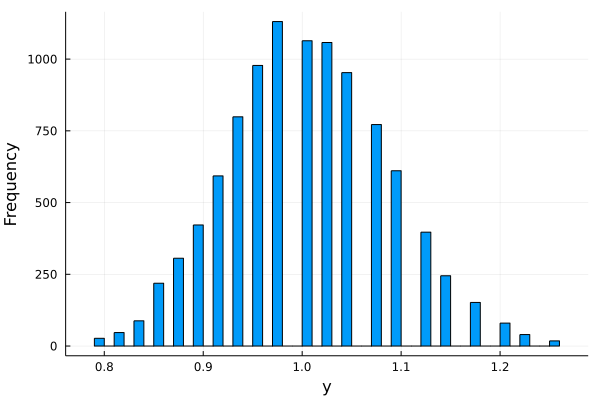
\includegraphics[scale=0.5]{endow_hist.png}
		\caption{Ergodic Distribution of Endowment}
	\end{figure}
	
	\begin{figure}[htbp]
		\centering
		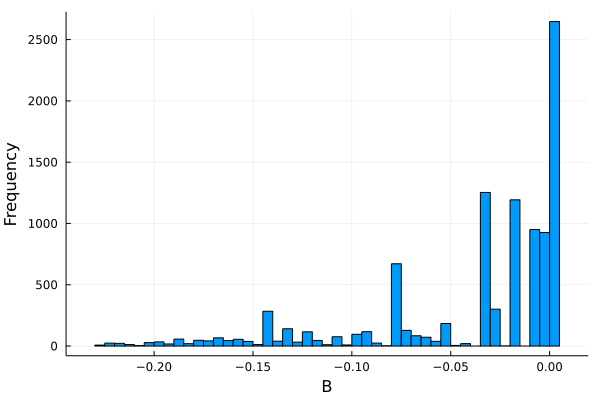
\includegraphics[scale=0.5]{B_hist.png}
		\caption{Ergodic Distribution of Asset (Debt)}
		\label{Fig2}
	\end{figure}
	
	\begin{figure}[htbp]
		\centering
		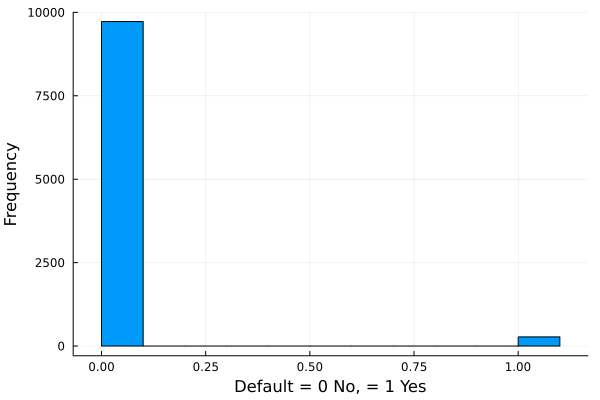
\includegraphics[scale=0.5]{default_hist.png}
		\caption{Ergodic Distribution of Default Choice}
	\end{figure}
	
	\noindent\textbf{Question 2:} Plot the marginal ergodic distribution of debt. What is the average level of debt? What is the maximum level of debt? \\
	
	\noindent\textbf{Solution:} For the marginal ergodic distribution of debt, see Figure \ref{Fig2}. From the simulated data, we find the average of an array of debt to be $-0.0379$ and the maximum level of debt to be $-0.2272$. \\
	
	\noindent\textbf{Question 3:} What fraction of time is the country in a default state? \\
	
	\noindent\textbf{Solution:} Given $T = 10000$, we check how many elements of the array of default states is equal to one. The answer is $275$. So the country is in a default state $2.75$ percent of the time. \\
	
	\noindent\textbf{Question 4:} What is the average output loss in default? \\
	
	\noindent\textbf{Solution:} The average output under not default is $1.0019$ while the average output under default is $0.941$. Therefore, the average output loss is $0.061$. \\
	
	\noindent\textbf{Question 5:} How does the answers above change if the cost of default is linear? That is, if $y_{D}(s_{t}) = 0.98 y(s_{t})$? (This is the value used in Aguiar-Gopinath (06))  \\
	
	\noindent\textbf{Solution:} After changing the cost of default, we plot the ergodic distributions of three variables of interest as follows:
	
	\begin{figure}[htbp]
		\centering
		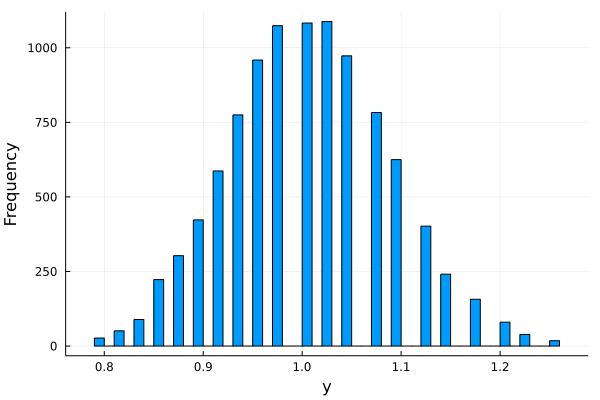
\includegraphics[scale=0.5]{endow_histQ5.png}
		\caption{Ergodic Distribution of Endowment}
	\end{figure}
	
	\begin{figure}[htbp]
		\centering
		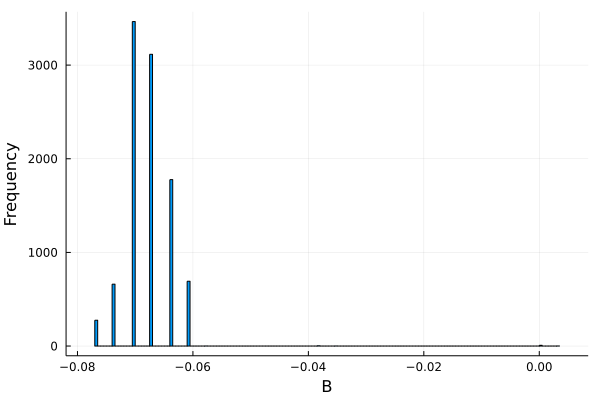
\includegraphics[scale=0.5]{B_histQ5.png}
		\caption{Ergodic Distribution of Asset (Debt)}
	\end{figure}
	
	\begin{figure}[htbp]
		\centering
		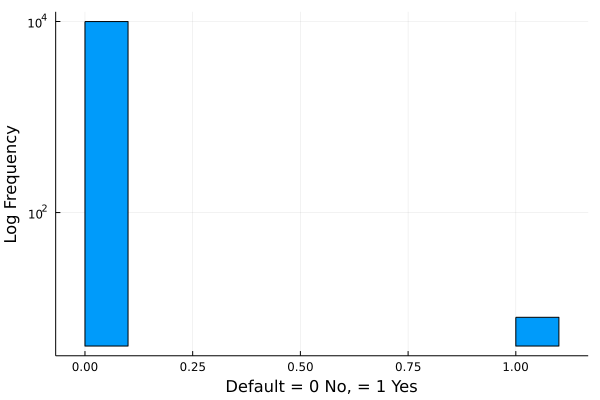
\includegraphics[scale=0.5]{default_histQ5.png}
		\caption{Ergodic Distribution of Default Choice}
	\end{figure}
	
	Comparing to the result under Arellano's setting, the distribution of endowment is not different as expected. The distribution of debt, however, is more concentrated and its range is much tighter than before. The average debt is $-0.068$, and the maximum debt is $-0.0768$. That is, the government borrows more on average, but keeps the debt at a lower level.
	
	Interestingly, compared to Arellano's setting, government tends to default less in this case. Out of $10000$ periods, only $8$ periods are in default and the average output loss is $0.112$. \\
	
	\noindent\textbf{Question 6:} Following from above, discuss the role of the non-linear default costs. \\
	
	\noindent\textbf{Solution:} To see the role of the non-linear default costs, we compare the plots of probability of default over $(B',y)$ under the two settings: Arellano's (Ar) and Aguiar-Gopinath (AG).
	
	\begin{figure}[htbp]
		\centering	
		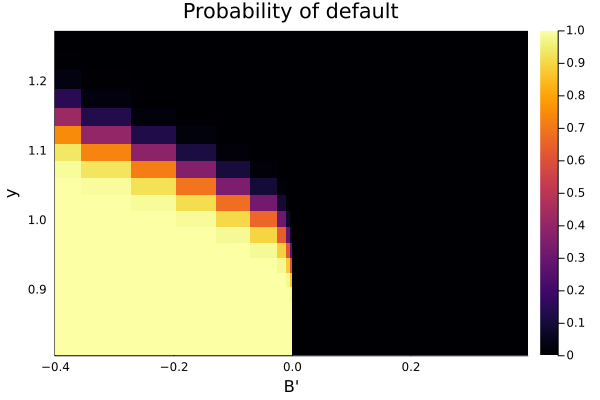
\includegraphics[scale=0.4]{PofD_Ar.png}
		\caption{Probability of Default over $(B',y)$, Arellano's Setting}
	\end{figure}
	
	\begin{figure}[htbp]
		\centering
		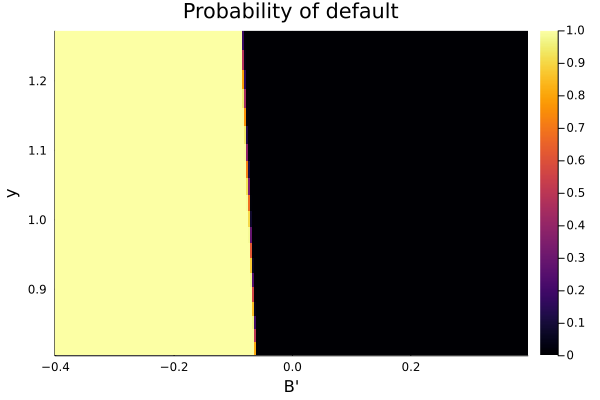
\includegraphics[scale=0.4]{PofD_AG.png}
		\caption{Probability of Default over $(B',y)$, Aguiar-Gopinath's Setting}
	\end{figure}
	
	Comparing to Ar's setting, the probability of default in AG's setting is much less sensitive to output. That is, given a level of debt B', the government's decision is almost always the same regardless of the level of output. This is because with the linear penalty in AG's setting, government at different states has almost the same probability of default. On the other hand, with the non-linear default cost in Ar's setting, default in good times is very costly, but much less costly in bad times. Hence we see the strong influence of output on the probability of default. \\
	
	\noindent\textbf{Question 7:} Consider now increasing the risk aversion coefficient so that $u = c^{1 - \gamma}/(1 - \gamma)$ with $\gamma = 10$. How do the implications of the model change? \\
	
	\noindent\textbf{Solution:} In this scenario, we change $\gamma$ from $2$ to $10$. Then the ergodic distribution of debt becomes
	
	\begin{figure}[htbp]
		\centering
		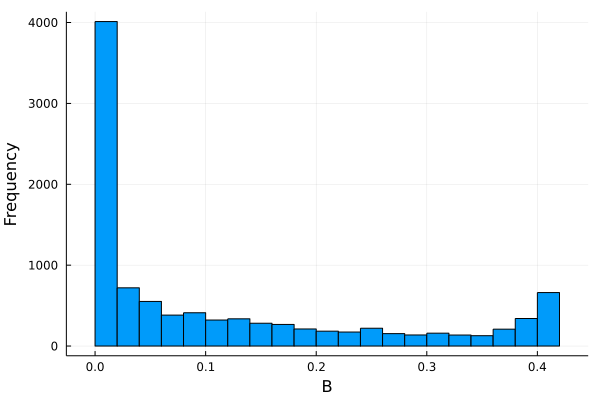
\includegraphics[scale=0.5]{B_histQ7.png}
		\caption{Ergodic Distribution of Debt, $\gamma = 10$}
	\end{figure}
	
	We can see that when $\gamma = 10$, the government does not borrow anymore. Instead it always choose to save with the mean of $0.116$ and the range of saving is $[0.0, 0.40]$. Since there is no borrowing, there will be no default.
	
	Because $\gamma$ measures the degree of risk aversion, the government with higher $\gamma$ is more risk-averse and since the government has a strong incentive to smooth consumption, it will save in good times.
	
	In bad times, it is true that government is more likely to default as the government is really painful when experiences a bad time under large $\gamma$. However, once default, the government will have to go through some uninsured periods, which will be more painful. Consequently, the government is always saving. \\
	
	\noindent\textbf{Question 8:} What happens if you make the government as patient as the foreign interest rate? What is now the debt level in the ergodic distribution? \\
	
	\noindent\textbf{Solution:} To make the government as patient as the foreign interest rate, we set $\beta = \frac{1}{1+r}$. Then the ergodic distribution of debt becomes
	
	\begin{figure}[htbp]
		\centering
		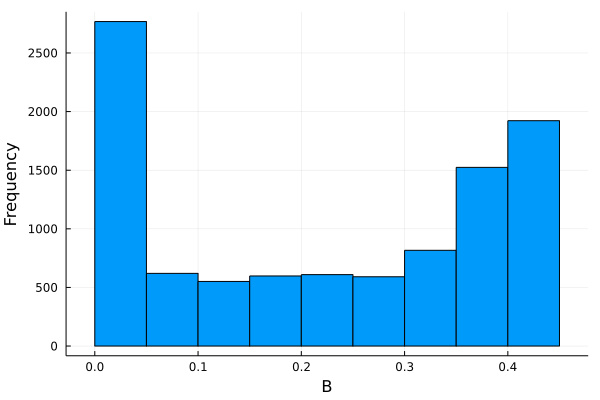
\includegraphics[scale=0.5]{B_histQ8.png}
		\caption{Ergodic Distribution of Debt, $\beta = \frac{1}{1+r}$}
	\end{figure}
	
	Again, the government does not borrow anymore and only chooses to save. The mean of saving is $0.216$ and the range of saving is $[0.0, 0.40]$. Because there is no borrowing, there will be no default. The reason is similar to that in Aiyagari $(1994)$. If $\beta(1+r) \ge 1$, consumption in the future will go to infinity, so the government will save in this case.
	
	
\end{document}